\documentclass[french]{article}
\usepackage[utf8]{inputenc}
\usepackage[T1]{fontenc}
\usepackage{pdfpages}
\usepackage{babel}
\usepackage{titlesec}
\usepackage{sectsty}
\usepackage{xcolor}
\usepackage{pst-all,pst-eucl}
\usepackage{hyperref}
\usepackage{ragged2e}
\usepackage{fancyhdr}
\usepackage{caption}

\definecolor{couleur_section}{RGB}{133,53,123}
\definecolor{couleur_subsection}{RGB}{0,99,111}
\definecolor{couleur_subsubsection}{RGB}{44,111,205}
\sectionfont{\color{couleur_section}}
\subsectionfont{\color{couleur_subsection} \hspace{0.4cm}}
\subsubsectionfont{\color{couleur_subsubsection} \itshape \hspace{1cm}}

\pagestyle{fancy}
\fancyhead{}%
\fancyfoot{}%
\definecolor{Couleur_pp}{RGB}{40,40,85}
\fancyfoot[C]{\color{Couleur_pp}\textit{\begin{center}Hashiwokakero - Jérémie Dautheribes - Camille Gosset \end{center} \newline} \thepage}
\renewcommand{\headrulewidth}{0pt}





\begin{document}

\begin{titlepage}
  \begin{center}
    % Institution et cursus
    
\includegraphics[scale=0.45]{logos.png}
    \vspace{1.5cm}
    
    \textsc{\LARGE Université de Montpellier}\\
    Licence~2 informatique\\
    HLIN405~--~Projet tutoré
    
    \vfill
    
    % Titre
    %\textsc{\Large Rapport de stage}
    %\vfill

 
    { \huge \bfseries Hashiwokakero - Projet Semestre impair \\[0.4cm] }

    %\HRule
    \vfill
    
    % Entreprise du stage
    %\emph{Entreprise~:} Point Course
    
    \vfill

    % Auteur et tuteur
    \begin{minipage}{0.9\textwidth}

        \center Camille Gosset - Jérémie Dautheribes       
    \end{minipage}

    \vfill

    % Dates 
    {\large Janvier - Avril 2017}
  \end{center}
\end{titlepage}



\section{\LARGE Introduction}
\hspace{0.5cm} Dans le cadre de l'unité d'enseignement de projet tutoré (HLIN405), nous avons développé en équipe le résolveur du jeu «Hashiwokakero». Notre groupe est composé de deux personnes: Camille Gosset et Jérémie Dautheribes.
L’objectif de ce projet est  de programmer un résolveur du jeu Hashiwokakero fonctionnel. Ce résolveur mobilise les bases d’algorithmique et de programmation apprises au cours de la première et deuxième année ainsi que nos connaissances et nos recherches personnelles. La création de ce résolveur nous a permis de renforcer nos capacités de travail en collaboration, en communication et en gestion de projet en général.
    \subsection{\Large Présentation}
    \hspace{0.5 cm} Hashiwokakero est un casse-tête représenté par une grille sur laquelle des des îles sont réparties. \`A chaque île est associée une valeur (entre 1 et 8). Le but consiste à relier les îles par des ponts de la manière suivante:
    \begin{itemize}
        \item 2 îles peuvent être réliées par 1 ou 2 ponts
        \item Chaque pont doit être vertical ou horizontal 
        \item Un pont ne peut traverser ni une île, ni un autre pont
        \item Le nombre de ponts issus d'une île doit être égal à la valeur de l'île
        \item Le réseau doit être connexe: toute île doit être accessible par n'importe quelle autre île
    \end{itemize}
    Sur la figure suivante, voici un exemple du casse-tête Hashiwokakero que l'on pourrait rencontrer dans un générateur du casse-tête classique.\\\\
    \centerline{\fbox {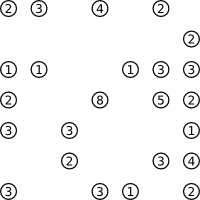
\includegraphics[width=0.3 \textwidth]{casconcret2.png}}}
    \captionof{figure}{Exemple de problème concret avant résolution}
    \label{exempleconcret}
    \centerline{\fbox{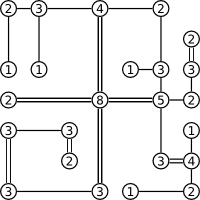
\includegraphics[width=0.3\textwidth]{casconcret.png}}}
    \captionof{figure}{Resolution du problème concret}
    \label{exempleconcretres}
    \vspace{0.5cm}
    Notre problématique consiste à reproduire la figure~\ref{exempleconcretres}: C'est à dire que nous avons pour objectif de construire la résolution d'une grille de Hashiwokakero générée aléatoirement.
    Nous avons remarqué qu'il y avait une corrélation entre le nombre de voisins possibles d'une île et le nombre de ponts restant à placer autour de cette même île.
    Par exemple: \\
    \centerline{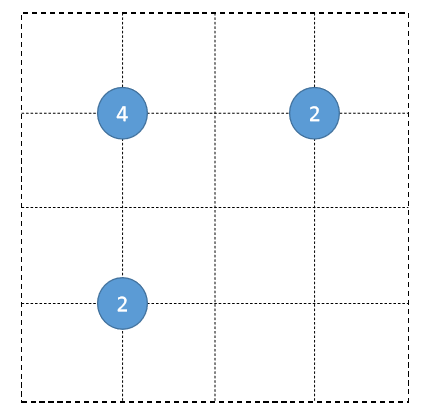
\includegraphics[width=0.3 \textwidth]{ExempleHashi.png}}
    \captionof{figure}{Exemple de problème (restreint)}
    \label{figure1}
    \vspace{0.5cm}  
    En effet sur la figure~\ref{figure1}, on constate la présence d'une île de valeur 4 qui a deux voisins possibles (qui ont chacun la valeur 2). Donc nous plaçons deux ponts sur chaque île, comme représenté sur la figure ci dessous:\\ 
    \centerline{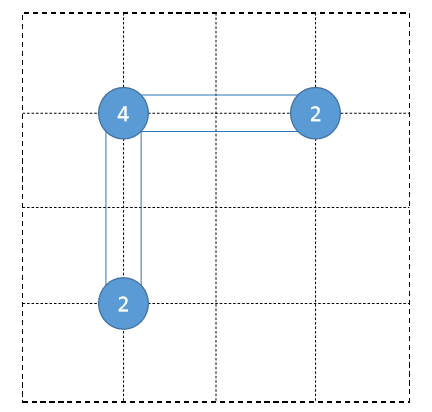
\includegraphics[width=0.3\textwidth]{ExempleHashiRes.png}}
    \captionof{figure}{Comment relier le problème}
    \label{figure2}
    \vspace{0.5cm}
   Notre première approche a consisté à définir des règles permettant de déduire l'existence de ponts et à les appliquer "en chaîne".
    \subsection{\Large Domaines de l'informatique}
    On peut distinguer deux domaines principaux sur lesquels notre projet a porté:
    \begin{itemize}
        \item l'algorithmique : Nous avons dû écrire nos algorithmes de la manière la plus efficace possible. Un problème NP est un problème dont la vérification de la solution est polynomiale. Un problème NP-complet est un problème qui est au moins aussi difficile que les autres problèmes NP et donc on peut se ramner à une réduction du problème déjà exploité. Dans notre cas, vérifier si une grille Hashiwokakero possède une solution est un problème NP-complet. C'est pourquoi, on ne peut pas espérer trouver un algorithme ayant une complexité inférieure à une complexité polynomiale. Nos connaissances en algorithmique ont été nécessaires pour ce projet mais celui-ci nous a aussi permis de nous améliorer dans ce domaine.
        \item la programmation : en effet, nous avons programmé notre projet en C$_+_+$ et nous avons crée une interface graphique à l'aide de la bibliothèque graphique SFML. Ce projet nous a également obligé à mobiliser nos compétences de programmation orientée objet acquises au cours du semestre précédent.
    \end{itemize}
   \subsection{\Large Cahier des Charges}
   Dans le cadre de ce projet il nous faut :
   \begin{itemize}
       \item Définir des types de données pour représenter les données d'un problème
       \item Réfléchir aux structures de données pour la résolution d'un casse-tête
       \item Ecrire des algorithmes de résolution d'un casse-tête et les programmer
       \item Expérimenter les différentes méthodes
       \item Faire une trace graphique d'une résolution
       \item Programmer le projet en C$_+_+$
   \end{itemize}
   
\section{\LARGE Organisation du projet}

    \subsection{\Large Organisation du travail}
        \subsubsection{Organisation et communication}
        \hspace{0.5cm} Pour répartir le travail, nous avons décidé de fonctionner par multiples réunions avec notre tuteur (chaque semaine). À l'issue de ces réunions, nous nous sommes attribués des tâches afin que chacun puisse avancer de son côté. Nous avons employé des outils de communication tels que Skype ou Appear (dont les liens sont dans la bibliographie) afin de communiquer en dehors des réunions et de s'entraider quand quelqu'un avait besoin d'aide.\newline
        \subsubsection{ Rigueur}
        \hspace{0.5cm} Nous avons immédiatement commencé le rapport et nous l'avons édité au fur et à mesure pour ne pas être dépassé. 
        Nous avons mis au point un document pour répertorier toutes nos méthodes et fonctions afin de voir si l'on s'en sert, combien de fois et à quel moment. Cela nous a donné la possibilité de déterminer l'importance de chaque fonction dans le code et ainsi savoir si l'on pouvait s'en passer. Ce document nous a permis d'épurer au maximum notre code et d'enlever plus rapidement toutes les méthodes dont on ne se servait pas. Nous avons fait régulièrement un nettoyage pour supprimer les éléments en trop, comme certains types de constructeurs  et d'accesseurs par exemple.
        \subsubsection{Affichage}
        \hspace{0.5cm} Nous avons commencé par un affichage basique afin de vérifier la bonne construction de notre grille ainsi que sa résolution. 
        Arrivés en fin de projet, nous nous sommes mis d'accord pour démarrer un affichage graphique plus élaboré: nous avons décidé d'utiliser la SFML, une interface de programmation graphique orientée objet. Notre choix s'est porté sur cette bibliothèque principalement graphique car nous l'avions déjà utilisée lors d'un précédent projet en première année de Licence.  De plus, elle a l'avantage d'être simple, gratuite et bien documentée en français.
    
    \subsection{Outils de développement}
    
    \hspace{0.5cm} Tout le code du programme est centralisé sur un dépôt GitLab de l'université (voir le lien dans la bibliographie) et les membres du groupe utilisent Git pour synchroniser leur travail, travailler indépendamment, vérifier le travail des autres ou récupérer d’anciennes versions.
    Nous avons fait le choix de la SFML comme bibliothèque pour l'affichage par fenêtre. 
    Pour écrire le code, nous avons utilisé différents éditeurs de texte (atom et emacs). Le compilateur choisi était g++. Nous avons utilisé gdb comme outil de débogage. Pour faciliter la compilation, nous avons utilisé Makefile. Enfin, nous avons utilisé le logiciel Valgrind afin d'identifier les fuites mémoires et autres pointeurs sur zones non allouées. \newline
    Pour obtenir un code homogène, nous nous sommes donnés des styles de codes: nous avons utilisé quatre espaces en guise d'indentation. En ce qui concerne les commentaires nous avons fait le choix de les faire en français. Les noms de variables et de fonction sont aussi en français mais les accesseurs doivent être précédés de set ou de get. Nous avons établi plusieurs styles de nommage: camel case supérieur pour les classes (ex: MaClasse), camel case inférieur pour les fonctions et méthodes (ex: maFonction), autre pour les variables (ex: ma\_variable), attributs privés précédés de \_. Les entêtes ne devaient pas contenir de code. \newpage
\section{\LARGE Analyse du projet}
    \subsection{\Large Découpage du code}
    \hspace{0.5cm} Nous avons découpé le code selon les quatre classes suivantes:
        \begin{itemize}
        \item Grille.hpp
        \item IleOuPont.hpp
        \item Ile.hpp
        \item Pont.hpp
        
        \end{itemize}
    Nous avons tout d'abord fait un diagramme d'UML (voir figure~\ref{uml}). \\
    \centerline{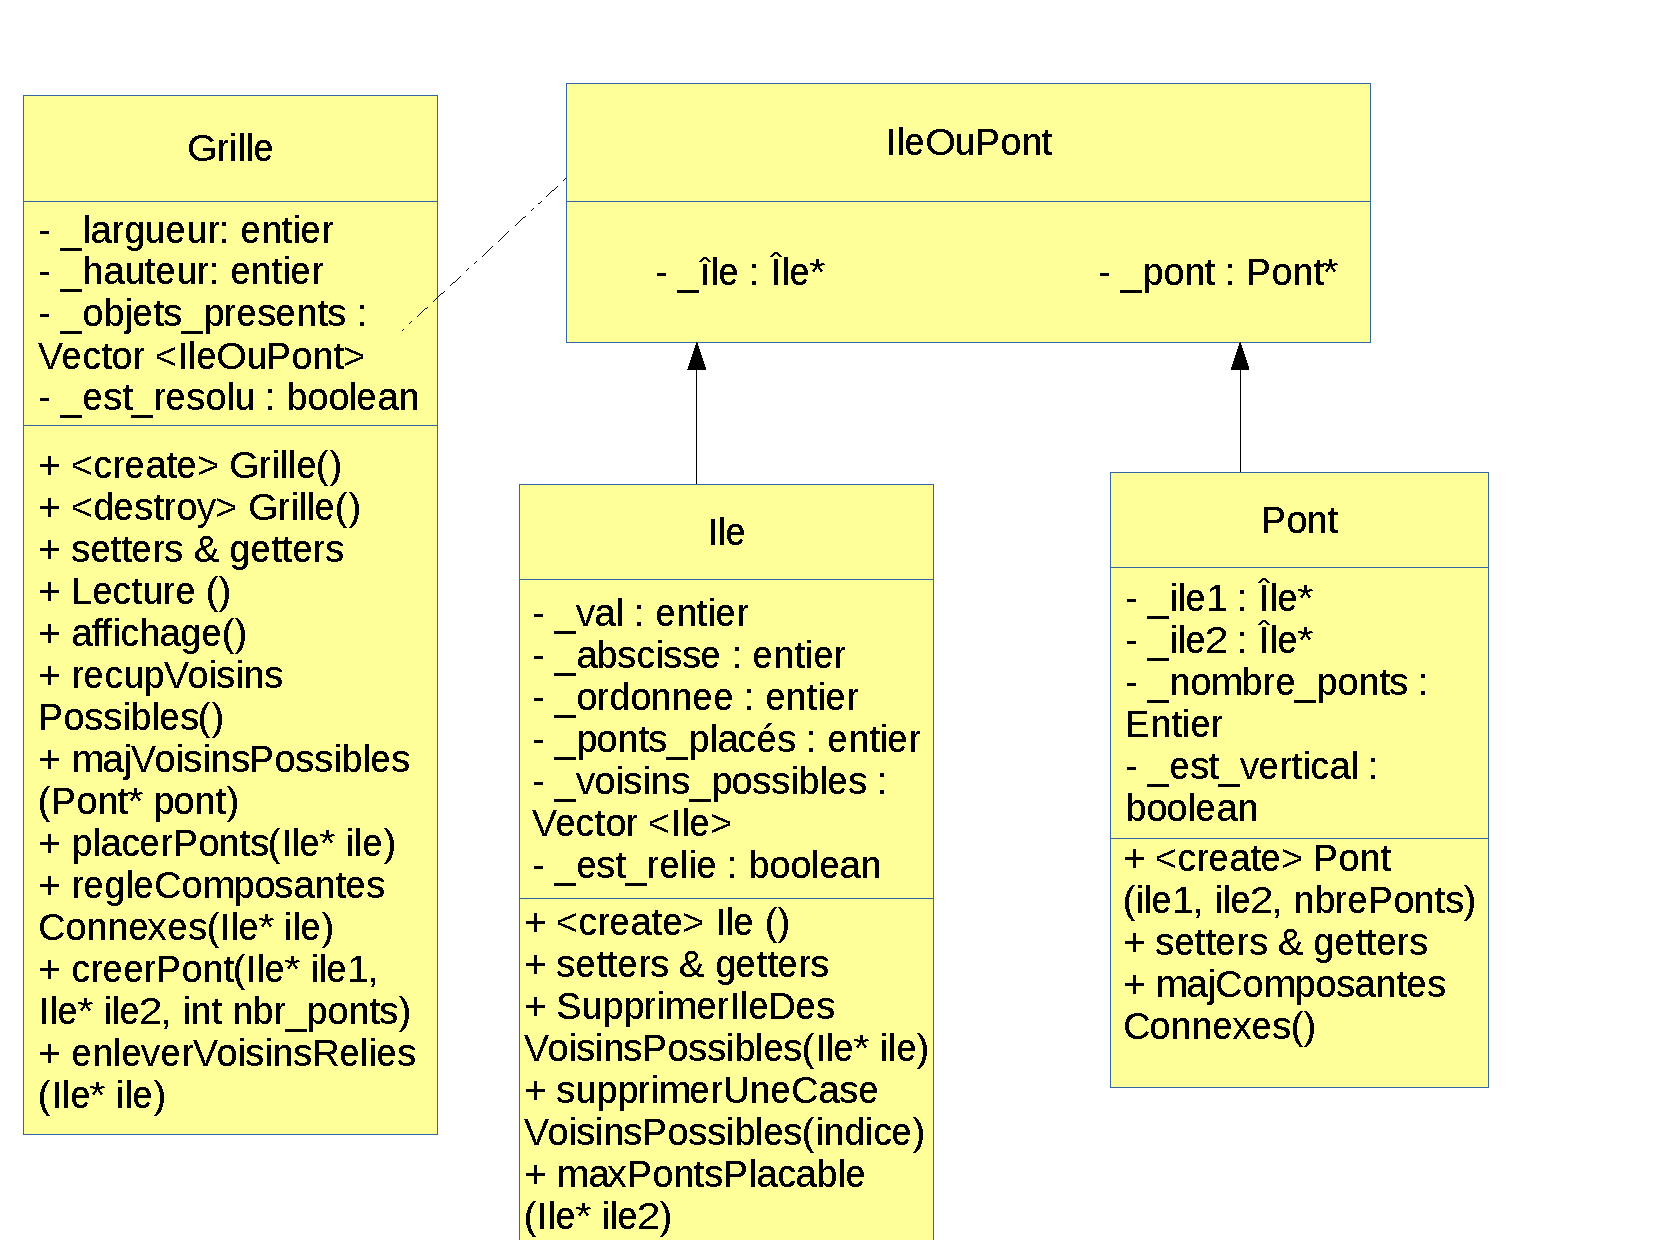
\includegraphics[width=1.1 \textwidth]{UML.pdf}}
    \captionof{figure}{UML des classes du jeu}
    \label{uml}
    \vspace{0.5cm}
 Notre UML se base sur une grille générale composée d'objets : pour chaque case (x,y) de la grille, on a soit un pont, soit une île ou soit une case vide. On a donc une super classe "IleOuPont" de laquelle trois cas peuvent être distingués:
 \begin{itemize}
     \item L'objet est à NULL. Il n'y a ni île, ni pont sur la case. C'est donc une case vide. Les deux pointeurs sont à NULL.
     \item L'objet est une île (mais pas un pont, le pont est à NULL).
     \item L'objet est un pont (mais pas une île, l'île est à NULL).
 \end{itemize}
 Dans la classe Ile, nous avons des attributs et des méthodes à expliciter:
 \begin{itemize}
    \item \_ponts\_placés: cet attribut représente le nombre de ponts qui sont déjà connectés à l'île.
    \item \_voisins\_possibles: la liste de toutes les îles qui seraient susceptibles de créer un pont avec l'île
    \item \_est\_relie: ce booléen est vrai si la valeur actuelle de l'île est à 0, faux sinon
    \item supprimerIleDesVoisinsPossibles(Ile* île): Cette méthode sert à supprimer une île des voisins possibles d'une autre île
    \item supprimerUneCaseVoisinsPossibles(indice):Cette méthode prend en paramètres un indice qui est l'indice de l'île que l'on veut supprimer des voisins possibles.
    \item maxPontsPlacable(Ile* île2): Cette méthode calcule le nombre maximum de ponts que l'on peut placer entre 2 îles. \\
\end{itemize}
 Dans notre classe grille, nous avons plusieurs méthodes importantes:
 \begin{itemize}
     \item lecture(): Cette méthode permet de reconstruire la grille: l'algorithme consiste à récupérer les éléments nécessaires dans un fichier pour reconstituer la grille (Largeur, hauteur de la grille et les îles présentes).
     \item recupVoisinsPossibles(): Cette méthode permet, en début de programme, de donner à chaque île la liste de ses voisins possibles.
     \item majVoisinsPossibles(Pont* pont): Cette méthode enlève des voisins possibles toutes les îles qui ont été séparées par un pont, les îles reliées et/ou les îles interconnectés par deux ponts.
     \item placerPonts(Ile* île): Cette méthode prend une île en paramètre et vérifie si des règles définies (pour la résolution) sont applicables.
     \item regleComposantesConnexes(Ile* île): Cette méthode vérifie si la règle des composantes connexes est applicable (elle est appelée en fin de programme)
     \item creerPont(Ile* île1, Ile* île2, int nbr\_ponts): Cette méthode permet de créer un nombre de ponts entre 2 îles (soit 1, soit 2) de valeur nbr\_ponts. Si un pont est déjà présent entre les deux îles, on double ce pont, sinon on le crée et on appelle majVoisinsPossibles(Pont* pont);
     \item enleverVoisinsRelies(Ile* île): Cette méthode enlève à chaque voisin l'île si elle est reliée et met les voisins possibles de cette île à null. Si cette île n'est pas reliée, alors on rappelle la méthode sur tous ses voisins possibles.
 \end{itemize}
\section{\LARGE Developpement et difficultées principales recontrées}
    \subsection{\Large Défnition du formalisme de fichier}
    \hspace{0.5cm} Tout d'abord notre tuteur nous a demandé de définir le format de fichier pour stocker les informations décrivant une grille de Hashiwokakero. Lors de la commande d'exécution de notre programme, ce fichier doit être passé en argument afin de pouvoir construire la configuration de notre casse-tête. \\
    Ce fichier est décrit dans la figure~\ref{syntaxeFichiers} ci-dessous. \newline
    \centerline{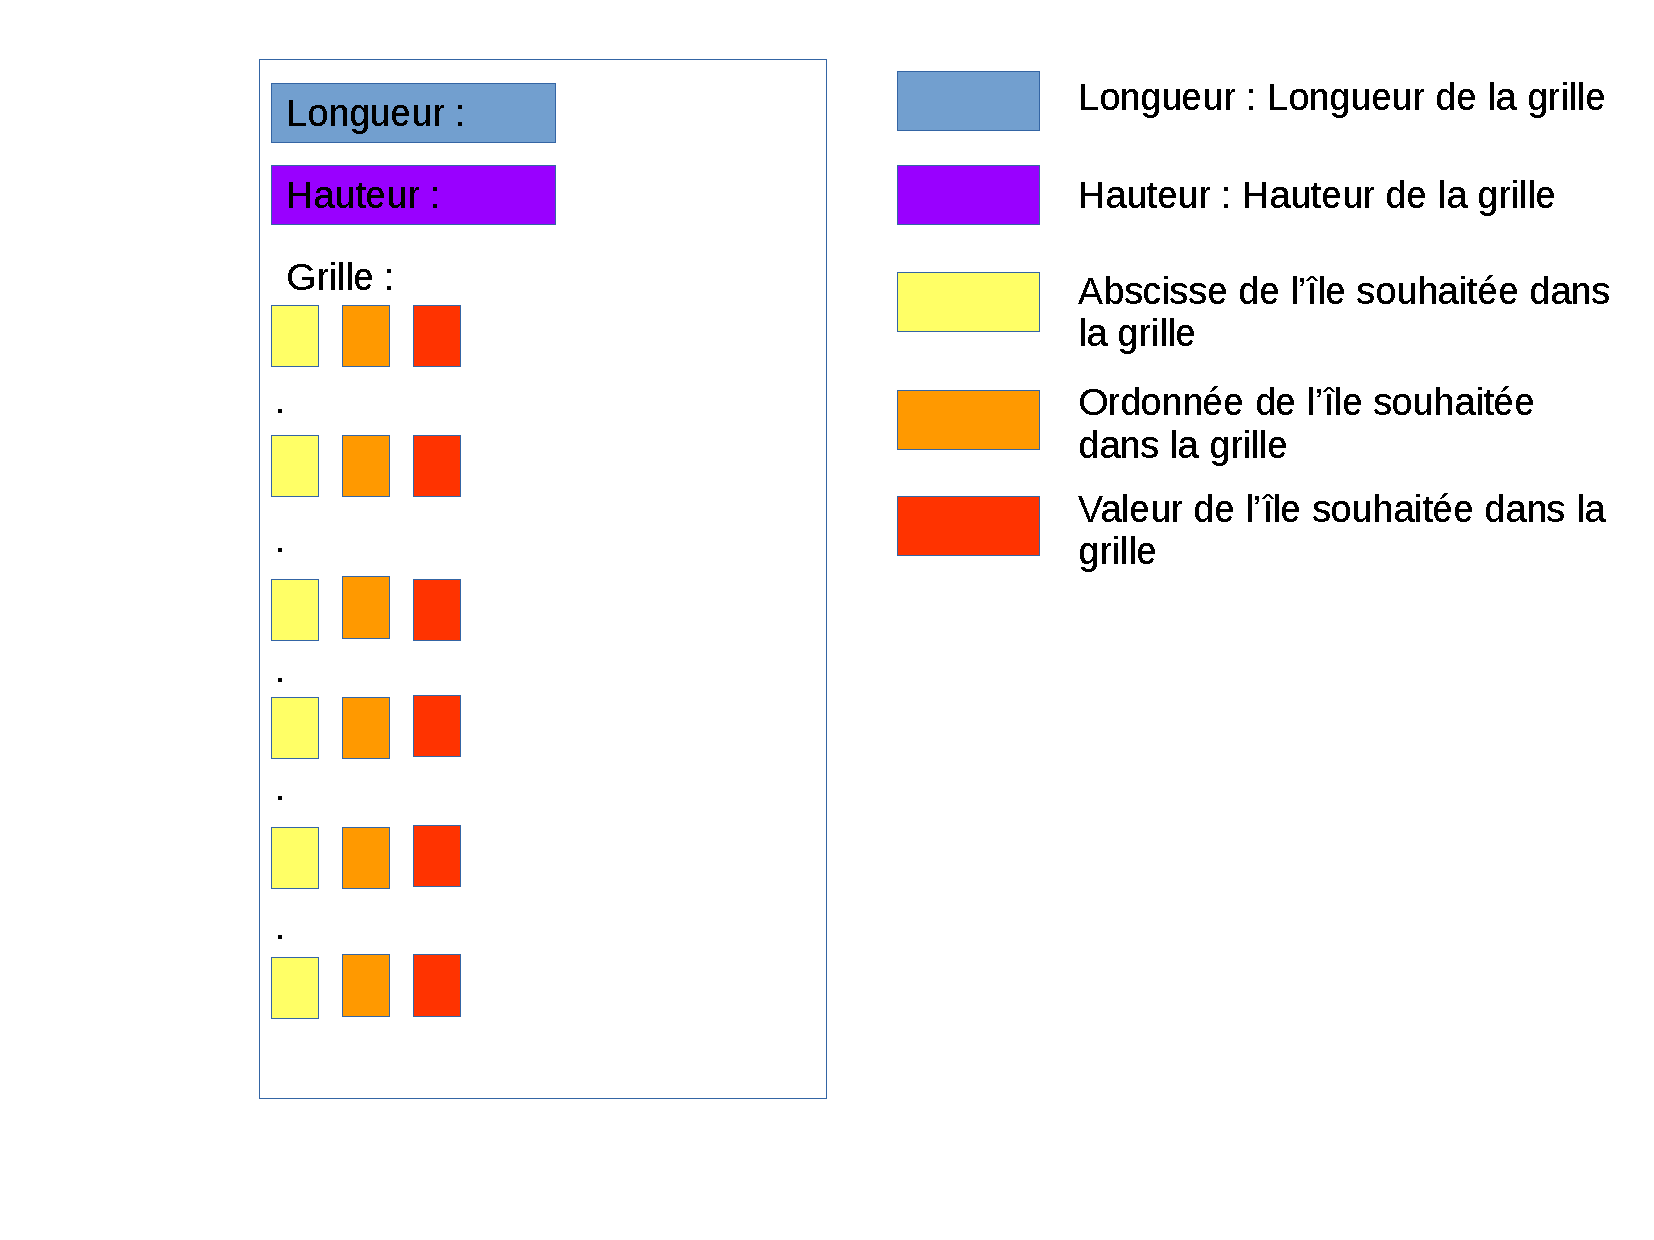
\includegraphics[width=1.3\textwidth]{Formalisme_du_jeu.pdf}}
    \captionof{figure}{Schéma de la syntaxe des fichiers}
    \label{syntaxeFichiers}
    \subsection{\Large Définition des classes de base}
    \hspace{0.5cm} Nous nous sommes d'abord occupés des classes principales : nous avons créé Ile, Grille et Pont. Nous avons commencé par réfléchir aux classes et ensuite on a codé le corps de la classe (constructeurs, accesseurs et méthodes principales). On a commencé par faire les entêtes pour être bien au clair avec le travail demandé et les fonctions que l'on comptait faire.
    \subsection{\Large Grille}
    \hspace{0.5cm} Nous avons changé de méthode: au début, nous étions parti sur un vecteur d'île qui était chargé de stocker toutes les îles présentes dans la grille et donc nous n'avions pas de réelle représentation de la grille. Or, nous en avons discuté avec notre tuteur et nous en avons conclu que nous allions devoir reparcourir tout le vecteur pour la moindre opération. Nous avons donc décidé de faire une grille d'île où les îles seraient placées dans la grille selon leurs coordonnées et l'accès aux îles serait plus simple. Nous avons ensuite décidé de faire une grille principale (tableau de tableaux) d'objets. On a donc créé un tableau de tableaux d'une nouvelle classe "IleOuPont" qui permet de modéliser les îles mais aussi de représenter les ponts au fur et à mesure de leur placement dans la grille.
    Par la suite, nous avons pensé rajouter un attribut: \_est\_vertical dans la classe Pont pour connaître la direction du pont.
    
    \subsection{\Large Coeur algorithmique}
    \hspace{0.5cm} Nous avons développé plusieurs méthodes importantes. Tout d'abord, nous avons déterminé des méthodes pour savoir les voisins possibles. Or, pour pouvoir développer ces méthodes, nous devions définir ce qu'est un voisin possible.
    Un voisin est possible s'il est sur le même axe que l'île et qu'il n'y a pas d'îles ou de ponts entre les deux îles. Ensuite nous avons créé une méthode qui place un pont. Cette méthode doit modifier les voisins possibles lorsqu'un pont est placé.
    Finalement, nous avons établi une formule générique pour énumérer les cas possibles.
    
    \subsection{\Large Cas généraux (et plus spécifiques)}
    \hspace{0.5cm} Pour résoudre le casse-tête, nous avons dû mettre au point des règles pour placer chaque pont. Nous avons un cas général mais pour plus de rapidité nous avons établi des cas plus spécifiques.
    \begin{itemize}
    \item Cas spécifique: Si aucun pont n'est encore placé on peut extraire deux cas: 
        \begin{enumerate}
             \item Si la valeur est paire et que l'île a un nombre de voisins possibles de moitié de cette valeur alors on peut placer deux ponts à chacun de ses voisins possibles.
            \item Si la valeur est impaire et que l'île a un nombre de voisins possibles qui vaut la moitié de cette valeur + 1 alors on peut placer 1 pont à chacun de ses voisins possibles.
        \end{enumerate}     
        \newline
    Nous avons constaté que ces règles pouvaient être modifiées pour en faire des cas généraux mais nous avons décidé de les laisser dans le code pour que la résolution soit plus rapide. En effet, il arrive que les règles générales ne se déclenchent pas alors que les règles plus spécifiques oui. Il faudrait attendre plus longtemps pour que les cas généraux s'appliquent.\\
    \item Cas généraux: nous définissons la variable \textit{max} comme étant le nombre maximal de ponts qu'une île peut placer à un instant donné.
        \begin{enumerate}
            \item Si la valeur actuelle (c'est à dire la valeur de l'île de départ à laquelle on enlève le nombre de ponts déjà placés) est égale \textit{max}, alors on place le nombre maximal de ponts autour de l'île.\\
            \newline
            {\centering 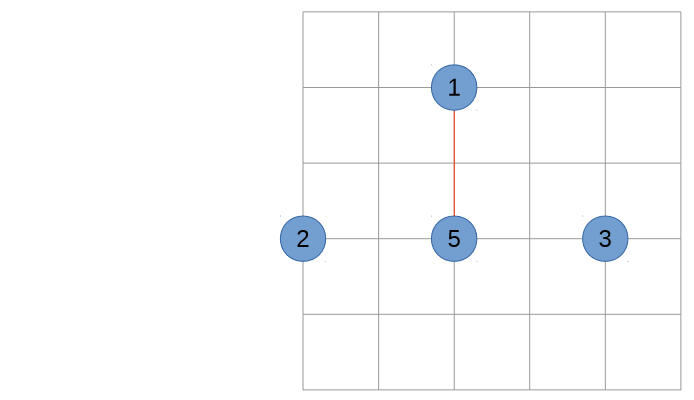
\includegraphics[width=0.6\textwidth]{Cas3a.png}}
            \captionof{figure}{Schéma d'un exemple du troisième cas (a)}
            \label{cas3a}
            \vspace{0.5cm}
            Comme on peut le voir sur la figure~\ref{cas3a}, on a déjà un pont placé. Donc l'île numéro 5 a une valeur actuelle de 4. 
            On constate qu'on a deux voisins possibles et en faisant la somme maximale des ponts que l'on peut placer, on obtient \textit{max} égal 4, ce qui correspond à la valeur actuelle de l'île (car on a sa voisine de gauche qui a une valeur actuelle de 2 et donc un nombre de ponts maximal à placer de 2 et de même pour sa voisine de droite qui a une valeur actuelle de 3). On peut donc placer deux ponts pour l'île numéro 2 et l'île numéro 3.
            \centerline{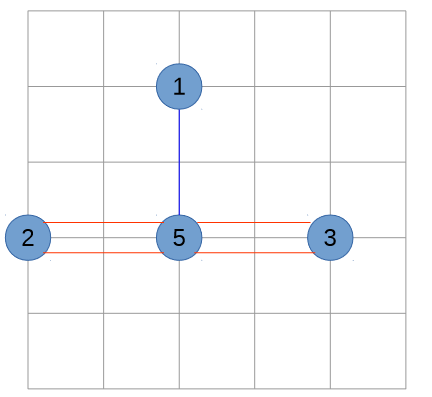
\includegraphics[width=0.4\textwidth]{Cas3aResolu.png}}
            \captionof{figure}{Schéma de la résolution de la figure~\ref{cas3a}}
            \label{cas3aRes} 
            \vspace{0.5cm}
            \item Si on a une valeur actuelle qui vaut \textit{max - 1} et qui est supérieure au nombre de voisins possibles, alors on crée un pont pour chaque voisin possible sauf les îles de valeur initiale 1. Si le pont existait déjà, alors on le double.\\
            \centerline{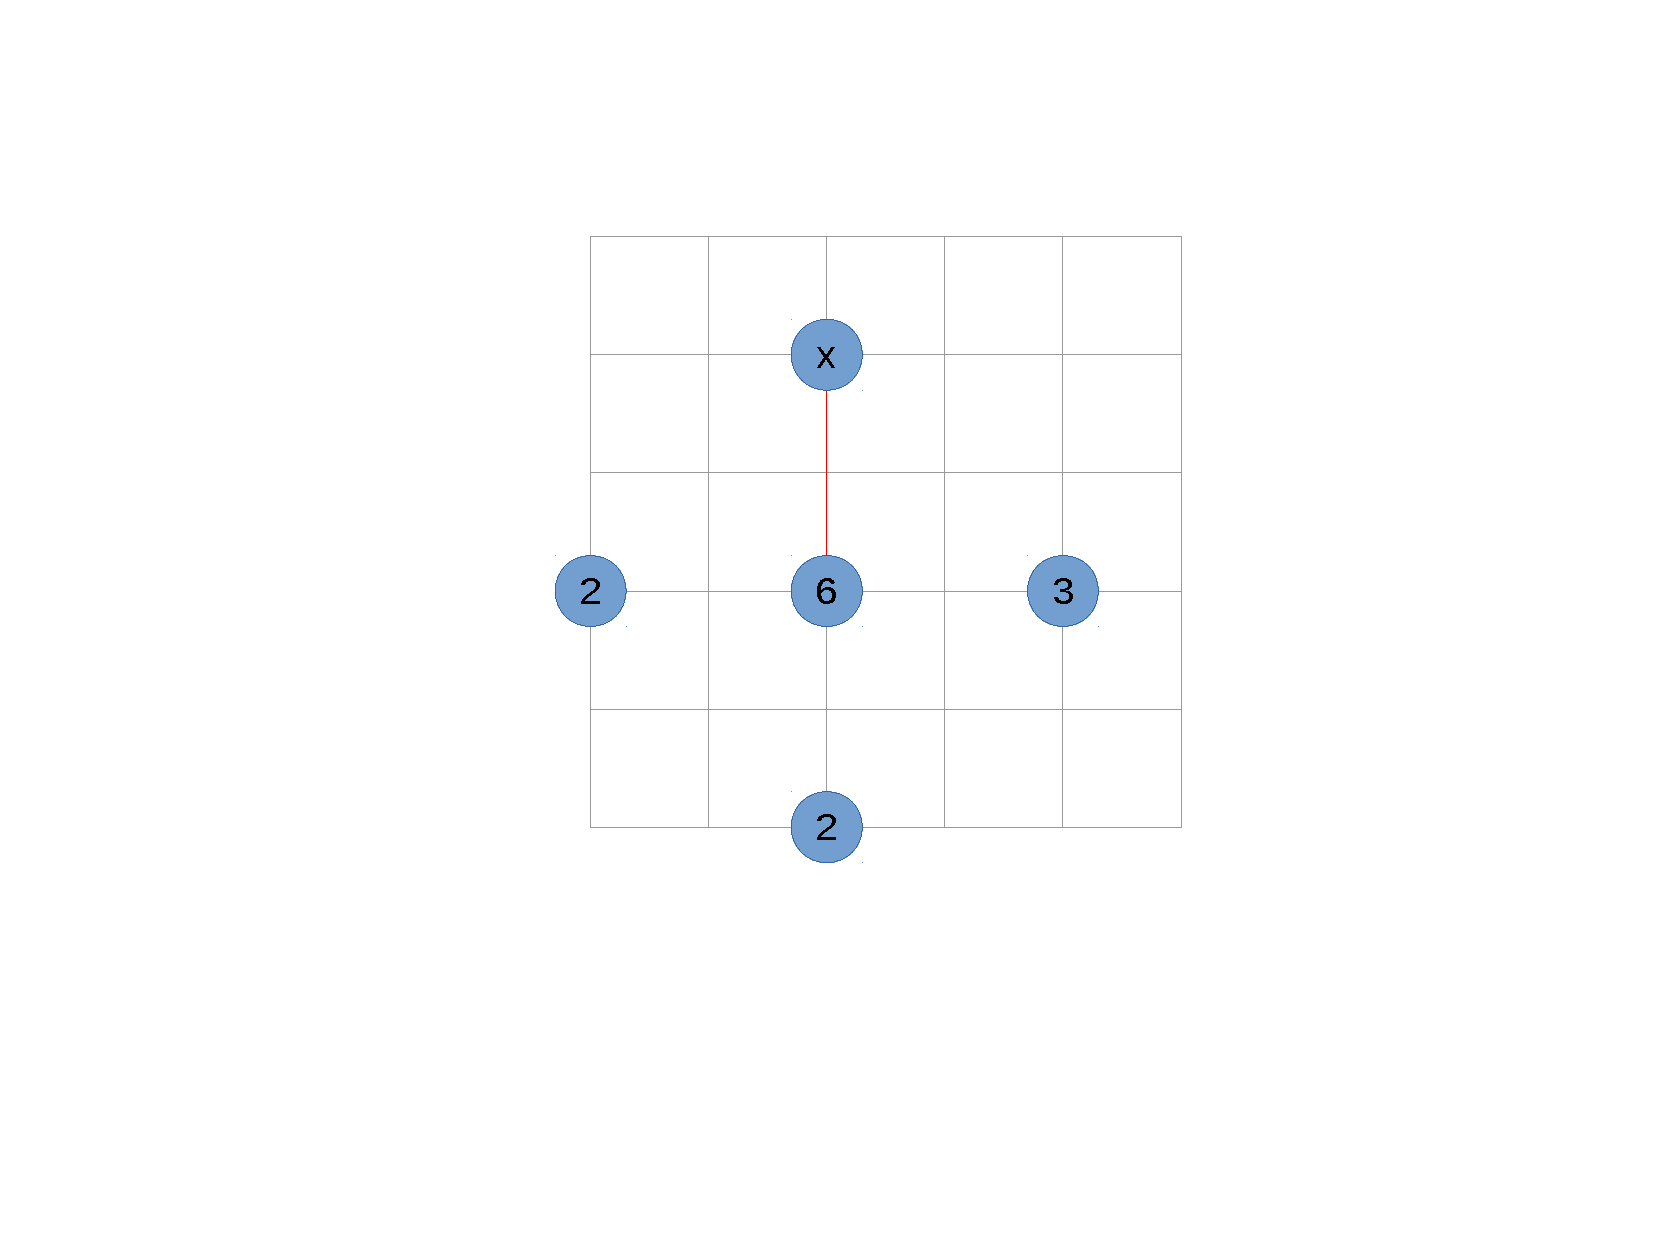
\includegraphics[width=0.8\textwidth]{Cas3b.pdf}}
            \captionof{figure}{Schéma d'un exemple du troisième cas (b)}
            \label{cas3b}
            \vspace{0.5cm}
            Comme on peut le constater sur la figure~\ref{cas3b}, on a déjà un pont placé provenant de x (qui doit avoir une valeur strictement suéprieure à 1) ce qui fait passer notre île du milieu à une valeur actuelle de 5. On a donc quatre voisins possibles avec une somme maximale de ponts plaçables de 6. On a donc une valeur actuelle égale à  \textit{max - 1}. On peut donc placer un pont partout.
            \centerline{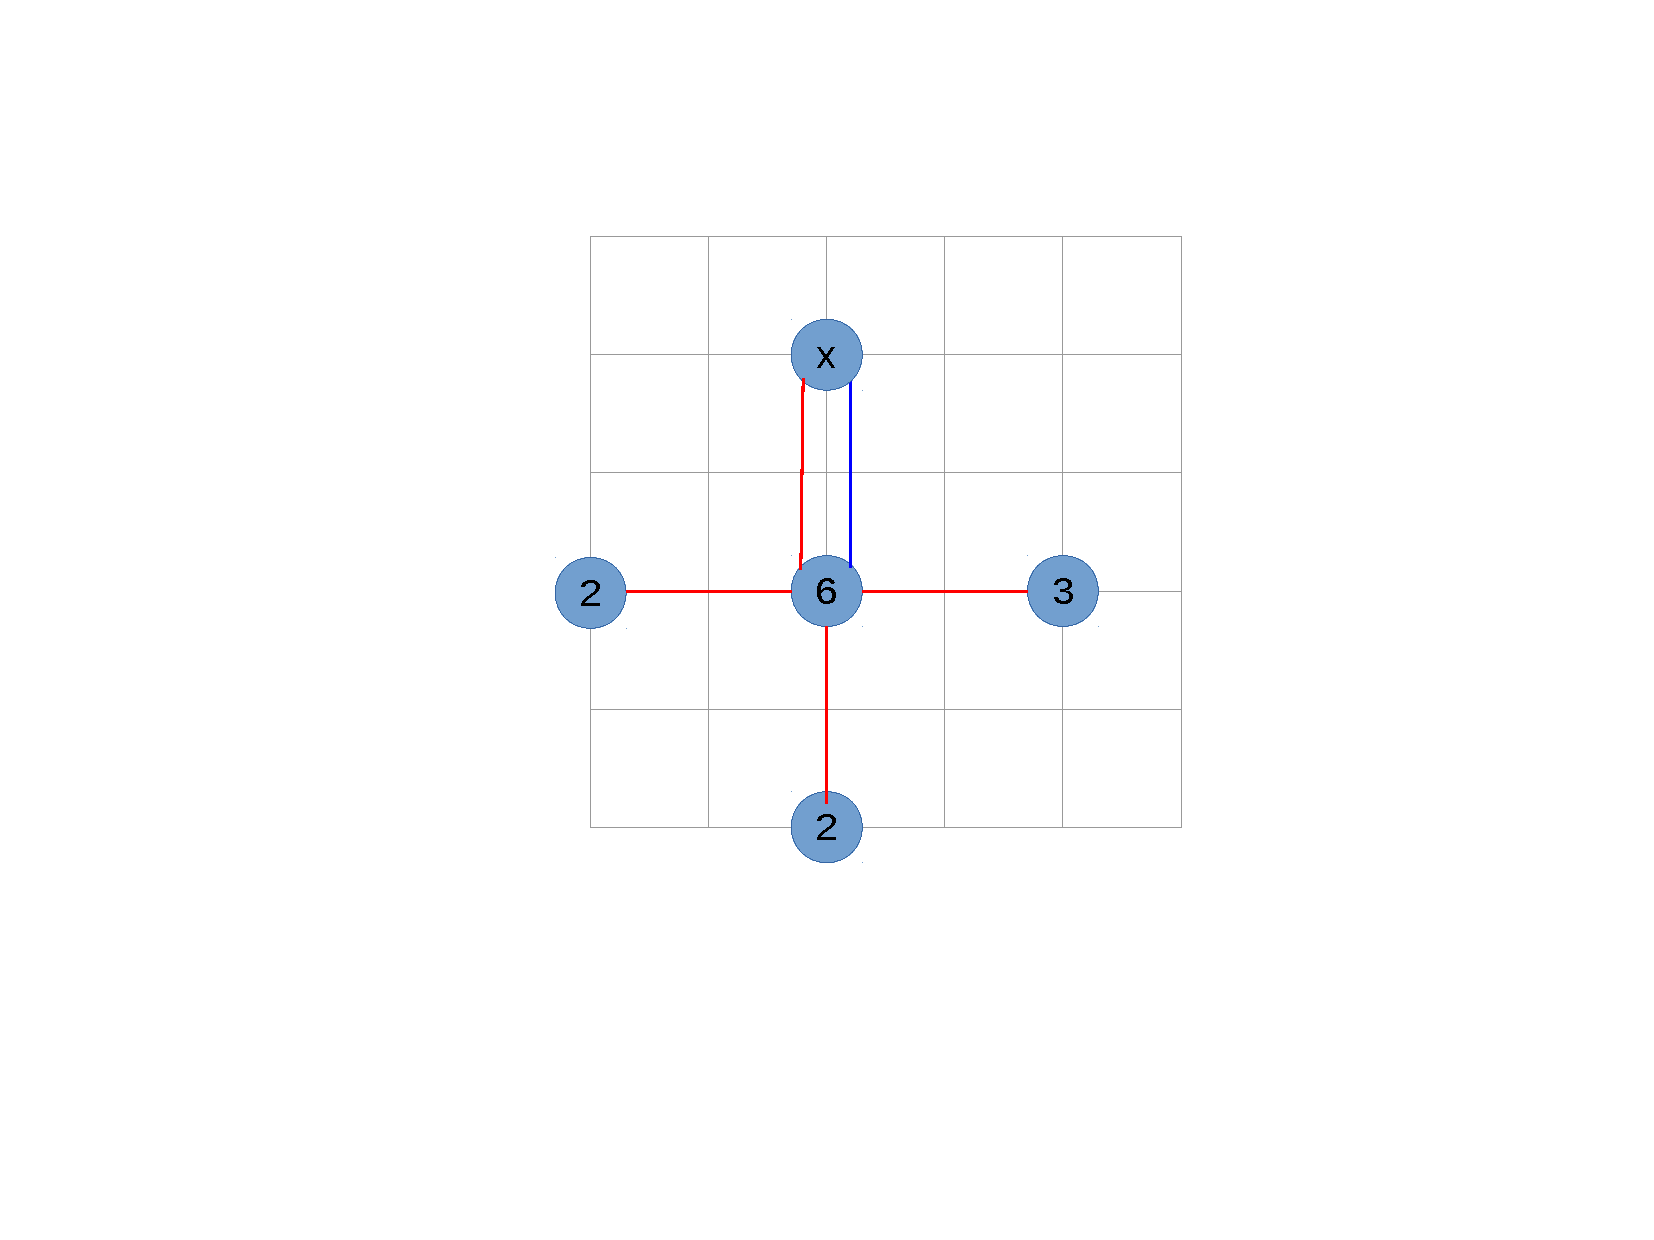
\includegraphics[width=0.8\textwidth]{Cas3bResolu.pdf}}
            \captionof{figure}{Schéma de la résolution de la figure~\ref{cas3b}}
            \label{cas3bRes} 
            \vspace{0.5cm}
        \end{enumerate}
    \end{itemize}
Enfin pour chaque règle déclenchée, notre algorithme repart du début de la grille pour vérifier si les règles peuvent s'appliquer à des îles précédemment analysées. \\
\newline
Il est important de noter que dans les configurations les plus complexes de Hashiwokakero, il n'est pas possible de placer tous les ponts en suivant uniquement ces règles. Il faudra au bout d'un moment obligatoirement placer certains ponts de manière aléatoire. 

    \subsection{\Large Mise à jour des voisins possibles}
    Cet algorithme (nommé majVoisinsPossibles(Pont*)) est appelé lorsque l'on place un pont. Cet algorithme consite à supprimer des voisins possibles les îles des deux côtés des ponts. Nous avons pour cela en paramètres un pont. Ensuite on cherche s'il y a 2 îles voisines de chaque côté et on les supprime du vecteur. \\
    Par exemple sur la figure suivante, on a un pont qui vient d'être placé.
    \centerline{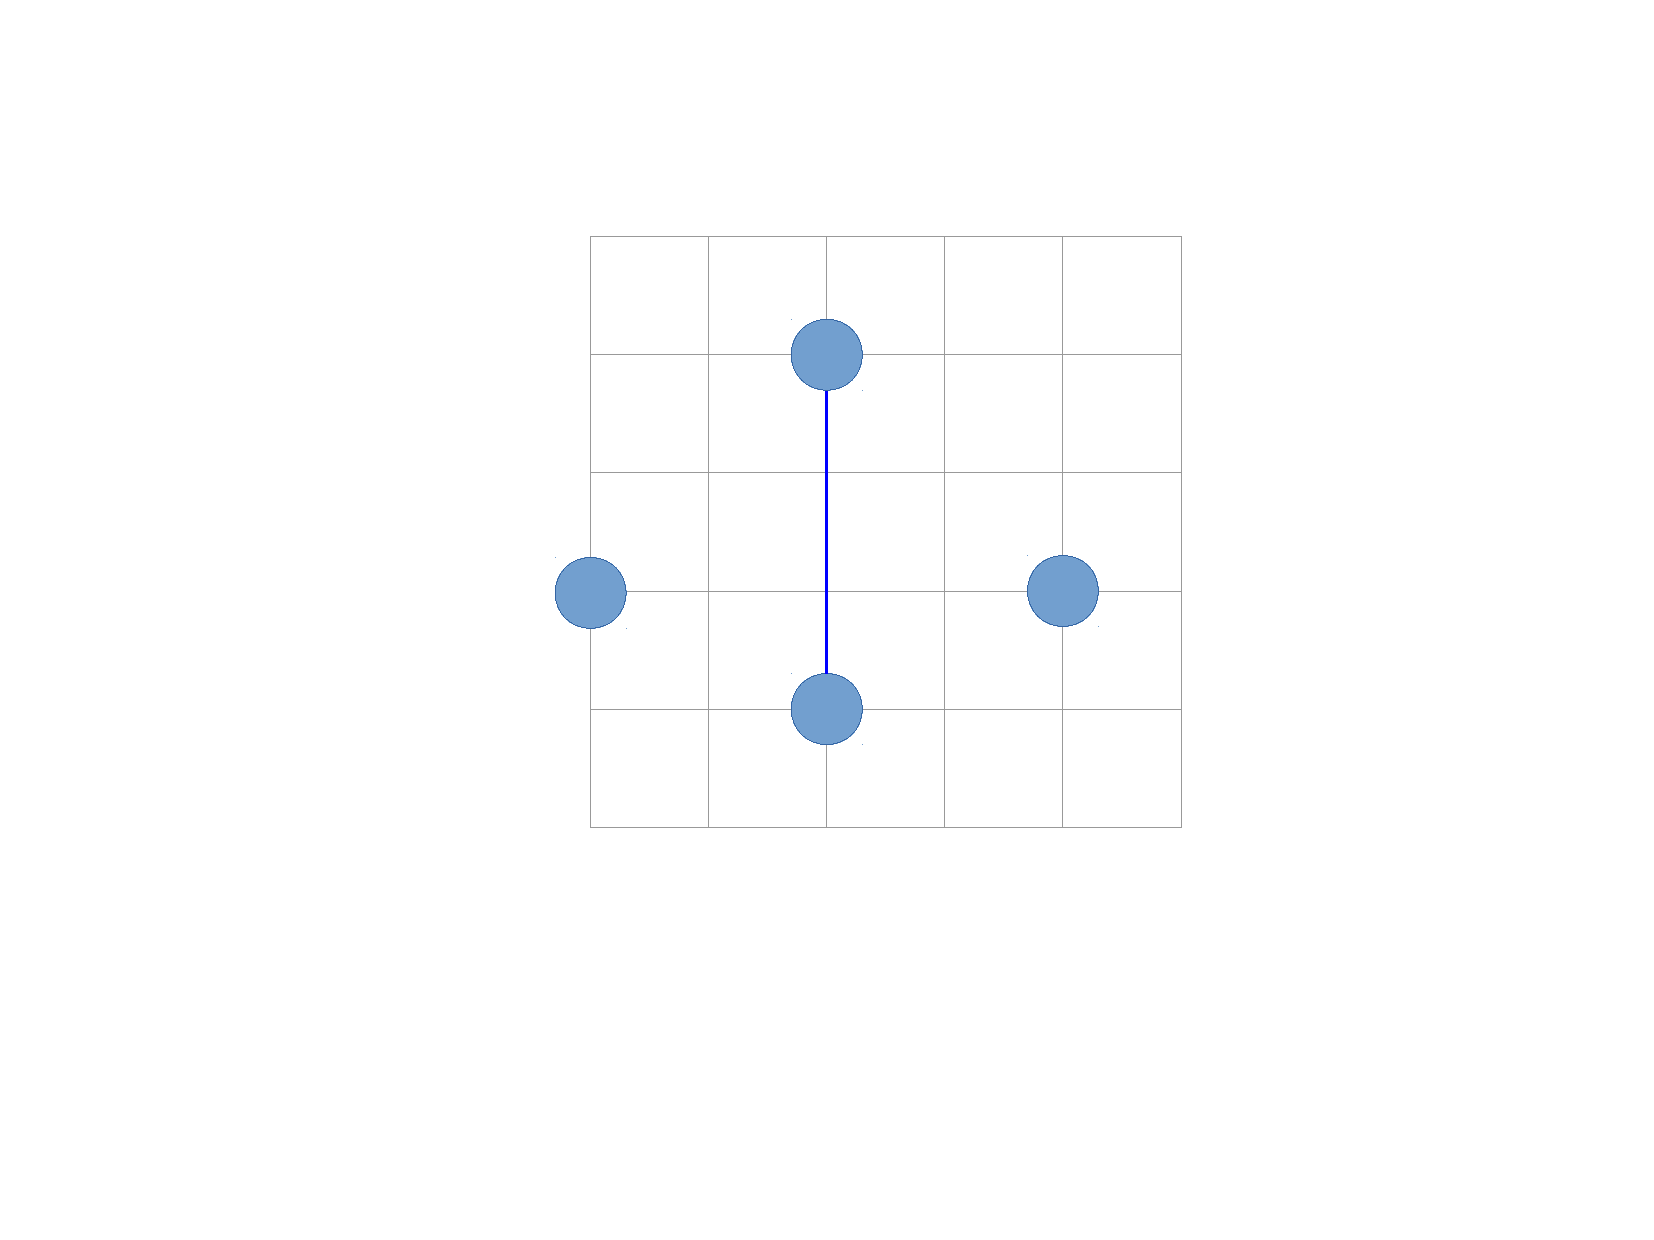
\includegraphics[width=0.8\textwidth]{majVP.pdf}}
    \captionof{figure}{Schéma d'un pont qui vient d'être placé}
    \label{majVP} 
    \vspace{0.5cm}
    Nous allons regarder de chaque côté si des îles étaient susceptibles d'être voisines et les supprimer de leur vecteur respectif (voir figure~\ref{majVPres}).
    \centerline{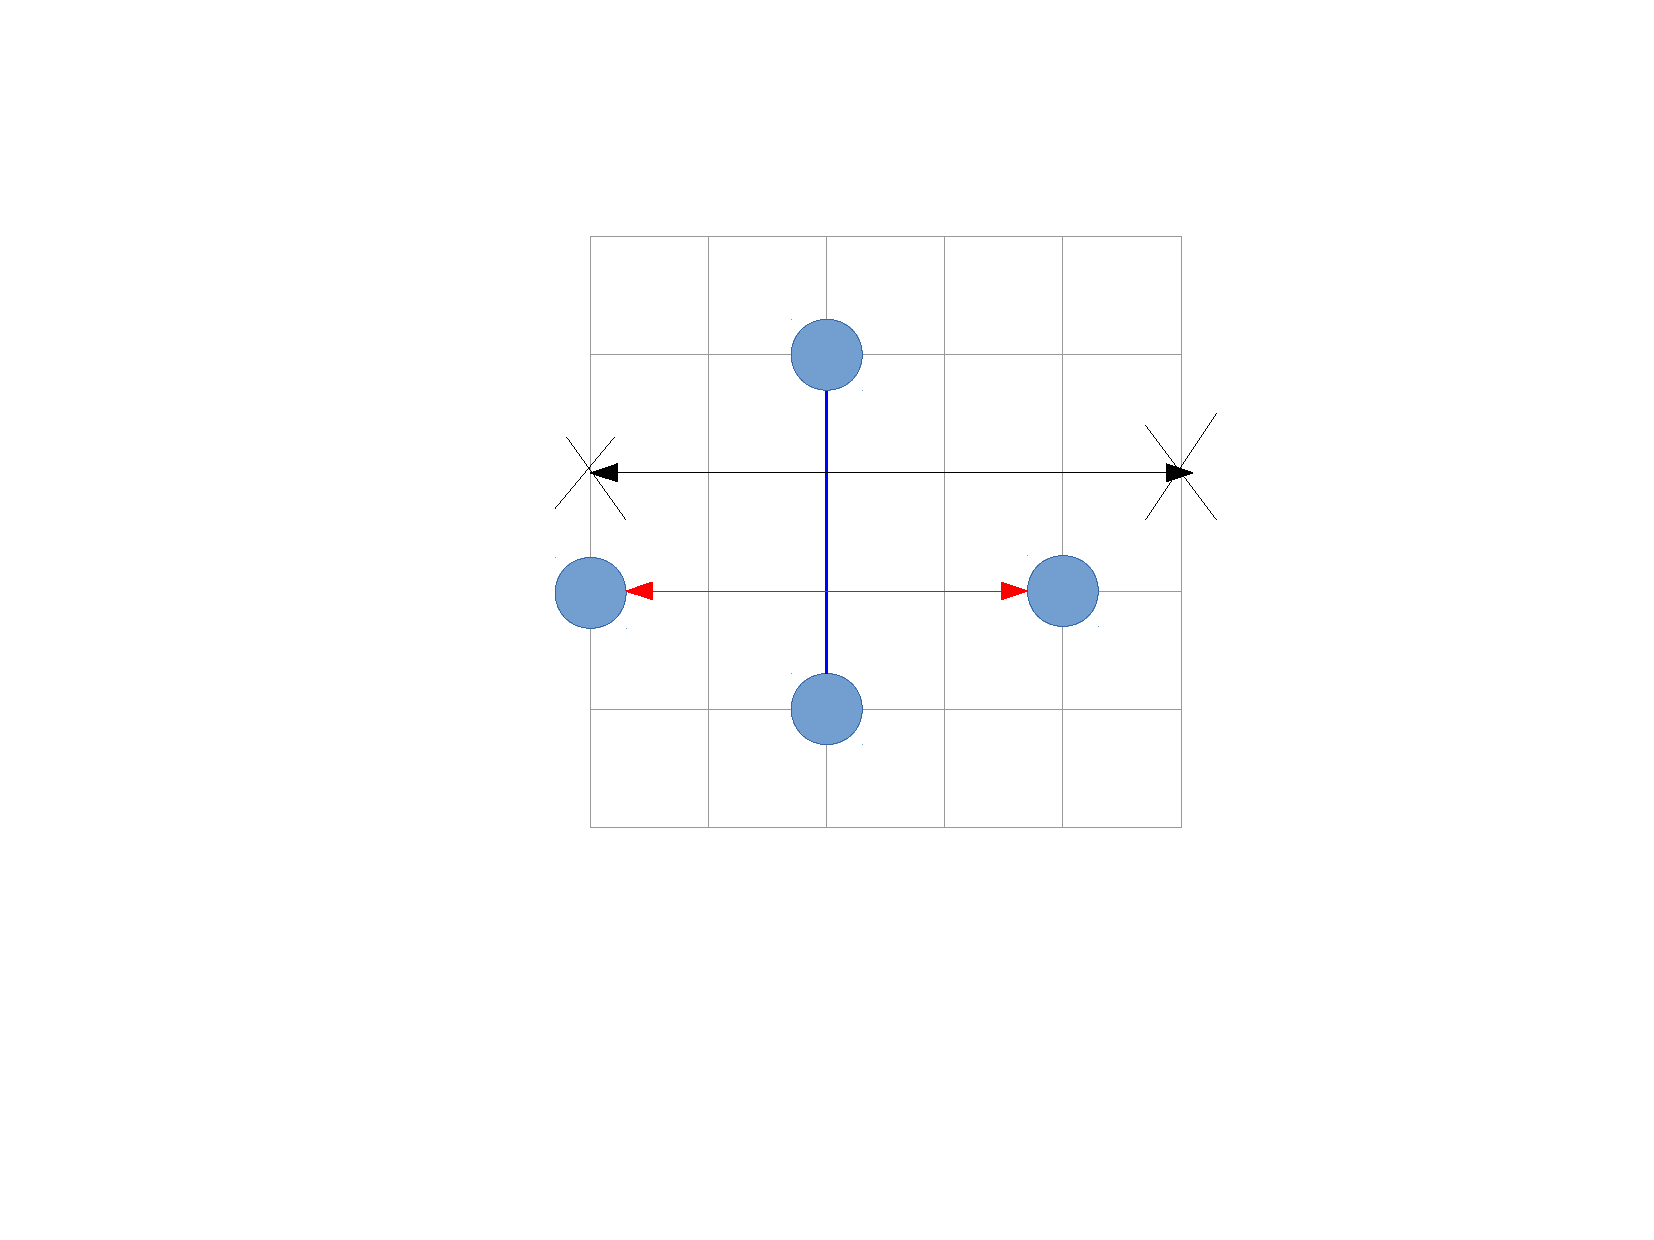
\includegraphics[width=0.8\textwidth]{majVPres.pdf}}
    \captionof{figure}{Schéma du parcours suite au placement d'un pont}
    \label{majVPres} 
    \vspace{0.5cm}
    Prenons notre figure de haut en bas. On peut constater que l'on fait notre parcours tout le long du pont. On fait un premier parcours en largeur et on ne tombe sur aucune île. Donc on descend le long du pont et là lors de notre parcours on tombe sur deux îles voisines. On peut donc les supprimer respectivement l'une des voisins possibles de l'autre.
        \subsection{\Large Composantes connexes}
    \hspace{0.5cm} Pour rappel, à la fin de la résolution du problème, les îles doivent appartenir à une seule et même composante connexe. Lors de la création de la grille, comme aucun pont n'est placé, on a autant de composantes connexes que d'îles. Lorsque l'on place un pont, si les îles n'appartiennent pas à la même composante connexe alors la structure des composantes connexes change: on doit faire l'union des composantes connexes. Pour faire cette union, nous avons pris le principe d'une bonne structure de données qui s'appelle l'union find qui consiste à mettre les composantes connexes sous forme d'arbre. Cette structure, nous l'avons découverte dans le chapitre sur l'union find d'un livre de François Schwarzentruber (voir bibliographie) donné par notre référent de projet. Chaque île fait partie d'une composante connexe sous forme d'arbre: toute île a un père sauf si l'île est chef. Un chef est la racine de l'arbre. Cet arbre a une hauteur qui est le plus long chemin entre le chef et les dernières îles de l'arbre.\\
    Nous avons donc ajouté à notre grille le nombre de composantes connexes en attribut puisque le problème est résolu quand le nombre de composantes connexes est égal à 1. Nous avons aussi ajouté dans chaque île une structure qui répertorie la hauteur de sa composante connexe, le père de l'île dans l'arbre ainsi que le chef de l'arbre. 
    Résoudre ce casse-tête en se servant des composantes connexes peut être productif. En effet, le but est de ne former qu'une seule et unique composante connexe. C'est pourquoi nous avons créé un algorithme que nous appelons en fin de résolution. Cette méthode consiste à parcourir les voisins possibles d'une île (appelée île1) et si parmi eux, il y a une unique île (appelée île2) qui ne fait pas partie de la même composante connexe que l'île1, alors on les relie.
\section{\LARGE Manuel d'utilisation}

\hspace{0.5cm} Afin de faciliter le processus de compilation au cours du développement du jeu, nous avons décidé de créer un fichier Makefile. \newline

Il est également nécessaire d'installer la bibliothèque SFML si ce n'est pas déjà fait.
Pour les distributions basés sur Debian, il faut exécuter la commande suivante : \newline
\noindent \texttt{sudo apt-get install libsfml-dev}

Pour la génération de l'executable, une fois placé dans le dossier Hashi, il faut exécuter la commande suivante dans le terminal : \texttt{make}

Une fois compilé, il faut se déplacer dans le sous-dossier \texttt{build} nous pouvons lancer le résolveur via \texttt{./Hashi}

Lorsque l'on lance le résolveur, nous devons passer un fichier en argument (fichier qui contient la configuration de la grille).
Par exemple, \texttt{./Hashi test.txt}
Ensuite nous n'avons qu'à attendre que le résolveur trouve une solution. Plusieurs fichiers de configuration sont présents dans le dossier build.
\section{\LARGE Conclusion}
    \subsection{\Large Perspective et apports}
    \hspace{0.5cm} Nous avions à notre disposition des créneaux pour rencontrer notre tuteur et pour se retrouver ce qui était une très bonne idée et ce qui nous a permis de bien avancer. \newline
    Les principaux points négatifs sont liés à la pression sur la dernière semaine.  Malgré tout, le ressenti global est positif grâce à une bonne entente dans l'équipe et à une bonne organsition. Cela nous a permis de confirmer et développer nos compétences en programmation C$_+_+$, en algorithmique, en gestion de projet et en gestion d'équipe.
    Nous n'avons pas fait de diagramme de Gantt ce qui aurait pu être un frein dans notre projet mais le fait que notre projet ait été tutoré nous a permis d'avoir un projet cadré grâce au planning que l'on se fixait chaque semaine .
    En ce qui concerne les futurs projets, nous envisageons de nous remettre ensemble en groupe pour d'autres projets. Nous envisageons cependant de faire un diagramme de Gantt et de faire régulièrement des tests logiciels (unitaires) vus en HLIN408 pour ne pas être bloqués en fin de projet et tester les fonctions au fur et à mesure comme nous avons pu l'être au cours du projet. Nous avons fait un diagramme UML de départ mais nous sommes restés sur un diagramme assez épuré. Nous aurions peut-être dû modifier au fur et à mesure le diagramme de Gantt avant de l'implémenter en C$_+_+$. Nous envisageons donc de faire un diagramme de Gantt évolutif pour nos futurs projets afin de comparer avec un diagramme épuré.
    \newline
    La plus importante perspective d'amélioration est l'implémentation d'un système de backtracking. Le backtracking, ou retour sur trace en français, consiste à revenir en arrière quand on arrive à une situation de blocage. Comme indiqué plus haut, notre résolveur n'applique -à l'heure où nous écrivons ces lignes- que des règles de résolution pour trouver la solution de la grille. Or, dans certains cas complexes, il est impossible de trouver une solution en appliquant simplement les règles. Il est nécessaire dans certains cas de placer les ponts d'une manière aléatoire. Et c'est ici que le système de backtracking entre en action: après avoir placé un pont de manière aléatoire, notre résolveur va appliquer de nouveaux les règles de résolution ou replacer un pont aléatoirement. Si ce ou ces placements de pont ne s'avèrent finalement pas bon, alors il faut revenir à l'état de la grille précédent le placement aléatoire du pont. Il faut donc placer ce pont à un autre endroit. Ce système peut être implémenté à l'aide d'une pile qui stocke les différents ajouts de pont aléatoires et qui permet ainsi de revenir facilement à une configuration précédente. Cela peut être également implémenté à l'aide de fonctions récursives qui jouent le rôle de pile. 
    \newline
    Enfin, une dernière petite amélioration consisterait à rajouter de l'héritage entre la classe IleOuPont et ses deux filles, Ile et Pont. En effet actuellement nous avons la grille qui est composée d'un tableau de tableaux d'objets, de la classe IleOuPont. Cette classe est composée de deux pointeurs, l'un pointant vers une île et l'autre vers un pont. Ce n'est pas la solution la plus jolie et la plus efficace (contrairement à l'héritage), mais nous n'avions à ce moment-là pas encore découvert la notion d'héritage. Cette compétence a été acquise durant le cours de HLIN406 et nous pourrions dans le futur intégrer l'héritage dans notre code. Nous aurions une classe Objet (ou IleouPont) dont les classes Ile et Pont hériteraient. Et la grille serait composée de case de classe Objet (ou IleOuPont).
    \subsection{\Large Conclusion}
        \subsubsection{\large Fonctionnement de l’application}
        \hspace{0.5cm} Nous avons rendu un résolveur qui fonctionne et nous avons rempli le cahier des charges demandé. Cependant, nous avons eu des contretemps qui nous ont retardé dans notre planning prévisionnel dans le développement du résolveur. Nous avons perdu beaucoup de temps du fait que nous avons voulu trouver des valeurs pour lesquelles le resolveur marchait (en terme de coordonnées) plutôt que de trouver le coeur du problème, le comprendre et le résoudre. Nous avons tout de même pu rendre un projet abouti.       
        \subsubsection{\large Fonctionnement du groupe de travail} 
        \hspace{0.5cm}Nous avons basé notre travail sur des réunions entre nous et avec notre tuteur (chaque semaine) ce qui nous a permis de gagner en efficacité du fait de notre répartition de travail. Si l’un de nous n’arrivait pas à effectuer sa tâche, il a pu demander de l’aide et facilement être conseillé. Nous avons programmé notre projet en C$_+_+$ et nous avons dû gérer des passages par pointeurs et par référence ce qui nous a permis d'augmenter notre niveau en programmation. En effet, nous avons rencontré des difficultées dues aux recopies des îles. Les îles n'étaient pas modifiées dans certains cas car on travailler sur une copies et non pas sur l'île en elle même. Cela nous a donc servis de leçon: nous savons désormais qu'il aurait été préférable de travailler principalement sur des pointeurs (notamment dans notre vecteur de voisins possibles) plutôt que sur des copies d'îles.
        Nous avons été un groupe de travail assez organisé du fait de nombreuses réunions et de nombreux plannings.
        Au niveau de la communication, nous n’avons eu aucun problème car nous sommes amis dans la vie quotidienne et, en plus de cela, nous nous retrouvions très souvent sur Skype ainsi qu’à l’université afin de discuter de tout problème. Cela nous a permis d'optimiser nos chances de trouver rapidement une solution.
        Enfin, grâce à notre motivation individuelle, une fois groupée et à laquelle on y ajoute une détermination et une coopération, nous avons pu aboutir à un projet fonctionnel tout en surmontant nos difficultés. Ce projet était l'une des premières étapes à notre formation et nous pourrons assuremment dans le futur réaliser de nouveaux projets plus longs et plus complexes. Nous avons également pour but de réaliser les perspectives pré-citées en vu de l'oral de notre projet.
        
\section{\LARGE Remerciements}
Nous tenons à remercier M. Janssen qui a été notre encadrant tout le long du projet et qui s'est vraiment investi dans notre projet tant au niveau du projet qu'au niveau du rapport.
Nous voudrions aussi remercier notre camarade et ami Matteo Delabre qui nous a permis de nous débloquer dans certaines impasses que nous rencontrions.
Nous voudrions aussi nous remercier l'un l'autre pour l'entraide que l'on s'est apportée mutuellement.
\section{\LARGE Bibliographie}
\begin{itemize}
    \item \url{http://www.xm1math.net/doculatex/}
    \item \url{http://www.cplusplus.com/reference/}
    \item \url{https://gitlab.info-ufr.univ-montp2.fr/}
    \item \url{https://www.skype.com/fr/}
    \item \url{https://appear.in/}
    \item Schwarzentruber, François. ALGO1 - ENS Rennes, chapitre 5 : Union find, p49-52
\end{itemize}
\end{document}
